%\documentclass[a4paper,twoside]{article}
\documentclass[a4paper, 10pt]{article}
\usepackage{graphicx}
\usepackage{rfia2000}
\usepackage[T1]{fontenc}
\usepackage{times}
\usepackage{multicol}
\usepackage{caption}
\renewcommand{\thefootnote}{\fnsymbol{footnote}}
\setlength{\parindent}{0.3cm}

\begin{document}
\long\def\/*#1*/{}
\date{}%{\today}
\title{\Large\bf Data Intensive processing with iRODS and the middleware CiGri for the Whisper project}
\author{\begin{tabular}[t]{c@{\extracolsep{8em}}c}
	Briand X.\footnote{Isterre, Cnrs, email xav.briand@gmail.com}  & Bzeznik B.\footnote{Ciment, Universit\'e Joseph Fourier} \\
\end{tabular}}

\maketitle
%\thispagestyle{empty}


\subsection*{Abstract}
{\em
blabla
\\
\\
\\
\\
\\
blabla
}
\subsection*{Keywords}
Data-Intensive, grid computing, distributed storage, Seismic Noise, Whisper, Cigri, Irods.



\begin{multicols}{2}
%\/*
\section{Plan}
\begin{enumerate}
	\item Introduction, abstract (3\S , 1 page) 
  	\item Background (7-10\S, 1-2 pages)
    \begin{enumerate}
  	  \item The Whisper project
  	  \item Size of observational data
  	  \item Size of computational data
  	  \item General Big data/ science of  universe
  	  \item Coupling scientific objectives / IT constraints
  	  \item Data grid paradigm
  	  \item Data grid in Grenoble
  	  %\item Whisper organisation
  	  \item Collaboration Whisper/IT infrastructure
  	\end{enumerate}
  	\item Software for data-intensive processing (6-12\S , 1-2 pages)
  	\begin{enumerate}
      \item General IT codes whisper
      \item Computer language and librairies
      \item Structure of codes
      \item Package for raw data
      \item Package for correlations
      \item First optimisation of correlation
      \item Second optimisation of correlation
      \item Codes for analysis of correlations
      \item Where we can run the codes
    \end{enumerate}
  \item IT infrastrcuture for grid computing (6-12\S , 1-2 pages)
    \begin{enumerate}
  	  \item Needs of coupling storage computation
  	  \item Presentation Ciment
  	  \item Coupling Irods/Cigri
  	  \item Resulting Data-Grid
      \item Presentation Irods
	  \item General Infra Irods (diagram)
	  \item Effective Nodes Irods (diagram)
  	  \item General Cigri
  	  \item Mechanism with OAR
  	  \item Mechanism resubmission/besteffort
  	  \item Description of a campaign
  	  \item Low Interaction Cigri/Irods
  	  \item Cigri V2 and V3 functionalities
  	\end{enumerate}
  \item Results (28-31\S, 6-7 pages)
  \item Discussion (7-10\S, 1-2 pages)
\end{enumerate}
%*/

\newpage
\section{Background 7-10\S, 1-2 pages}
~\\




The \emph{Whisper} \footnote{FP7 ERC Advanced grant 227507, see whisper.obs.ujf-grenoble.fr} 
project is a an european project on seismology whose goal is to study properties of the earth
with the seismic ambient noise such that evolution of seismic waves speed. 
This noise is almost all the signal continuously recorded by
the seismic stations worldwide (Europe, China, USA, Japan), except earthquakes. It offers new
observables for the seismologists, new types of virtuals seismograms that are not only located at the 
place of earthquakes. For instance, one can obtain wave paths that probes the deepest part of the Earth.
%(variations in space and time of the seismic waves)

 
Accordingly, this is one of the first project in the seismological community that studies
systematically the continuous recordings, which represents a large amount of seismological data, 
of the order of several tens of terabytes.
For instance, one year of the Japanese Network is about 20 TB or 3 months of the mobile network
USArray represents 500 GB (it depends on the sampling of the recorders).


In addition, the calculation operations downstream may produce even more data than the observation data.
To give an order of magnitude, more than 200 TB has been managed by the Whisper project at the same time. 
A classical processing produces 8 TB in 5 days. An other one 'read' 3 or 4 TB and 'produced' 1 TB in 6 hours.
Many tests of the signal processing are done and computational data are deleted as and when required.
\\


Nowadays, the earth sciences or more generally, sciences of the universe are widely engaged in
data-intensive processing. This leads to design scientific workflow, towards data-intensive discovery and e-Science.


Reflected by the Whisper project, we have to organize the science objectives with
the computer constraints. We have to take into account 
the duration of postdocs and PhD theses, as well as the availability of computer infrastructures and their ease of access. 
This leads to many questions about software development, including the genericity of computer code and 
the technical support. But it also influences in terms of choice of appropriate infrastrucures.

Even if this project has his own ressources, such a problem of data-intensive requires specific tools able to 
organize distributed data management and acces to computational ressources: a data grid environment.

The University of Grenoble offers, thanks to the High Performance Computing (HPC) centre \emph{Ciment}, this kind of environement with the distributed file system \emph{Irods}
and the middelware \emph{CiGri}.% (Ciment platform).


It is thanks to the close collaboration between IT ressources of Whisper and the infrastrucrures of the University
that this project has been implemented as we show below.


\newpage

\section{Software for data-intensive processing (6-12\S , 1-2 pages) }
~\\

A part of the Whisper project is specificaly dedicated to the IT codes. This includes to design a specification, an implementation and some optimisations of
a sequence of a data-management and of a computations \footnote{see code-whisper.isterre.fr/html/ (part of the design)}.
This project uses some own IT resources (servers, dedicated bay) but also uses common IT infrastructure of the university.
We developed also adaptations for the IT infrastrutures and we provide technical support for researchers.

Most of the IT codes are writing with the \emph{Python} language and uses intensively the scientific libraries \emph{Scipy} (fortran and C embeded) 
and \emph{Obspy} \footnote{ see www.obspy.org} (essentially the 'read' function). The latest one is dedicated to the seismological community. 

The IT codes consists of several tools described schematically at the figure \ref{whisperGeneralWorflow} and grouped into three parts. The first one concerns the signal processing, the second part permits the computation of the correlations and the last part consists of codes for the analysis of the correlations.

A first package provides a flexible way to process raw data, to specify a pipeline of pre-processing of signal.
The user starts by specifying a directory, a set of seismic stations and a set of dates. Then the codes scan the directory
and extracts all pieces of seismograms (also called traces) and rearranges them in a specific architecture of files in order to calculate the correlations to the next step.
We use here intensively the function 'read' of the library Obspy which allows to open most of format files seismogram.
The user also define his own sequence of processings. He can use the functions predefined but also the Python libraries he needs. 
Moreover he can add eventually his own processing.

The second package concerns correlations. Roughly speaking, a correlation is an operation with two seismograms that provides the coherence between the both signal (for a given time windows). Moreover, it represents, in some favorables cases, a new virtual seismogram (it converges to the Green's function). Thus, the code computes all the correlations and provides an architecture of files that corresponds to all the couples of seismograms (for each date). 

%\end{multicols}
\begin{center}%[h]
\centering
\captionof{figure}{\label{whisperCorrelationStep} Step of the correlations}
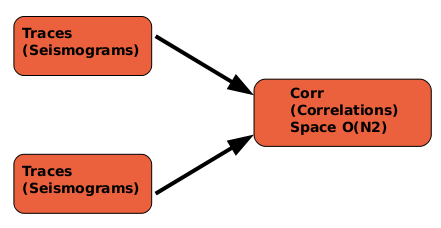
\includegraphics[width=6cm]{schemaCorrelationStep.png}
\end{center}
%\begin{multicols}{2}

These quadratic space complexity can be critical and lot of effort was made in order to optimize the computation in two direction. First we improve the computation of the fast fourier transform by pre-calculating some "good" combinations of small primes numbers. 
With this method, we improve of forty percent the time computation in the favorable cases.

Nevertheless, the main optimization was made by testing the behaviour of the carbage collector of Python in order to follow the cache heuristics. More precisely, we do not use the gc module or the 'del' statement but we try to schedule and localize the line of code in order to find the good unfolding that uses the architecture optimally.

The last part of computer codes concerns the analysis of correlations (the virtual new seismograms) with methods such as beamforming, doublet or inversion.
We also compute correlations of correlations C3 (also new seismograms). For example, we study the variations
in velocity of seismic waves as we illustrate below. 

These codes permit to process a dataset on a computer laptop. 
Nevertheless, to take advantage of IT infrastructure at the University of Grenoble, 
adjustments have been made for the grid computing as we shall see later.

\end{multicols}
\begin{figure}[h]
\centering
\caption{\label{whisperGeneralWorflow} Main sequences of processings of the Whisper Codes}
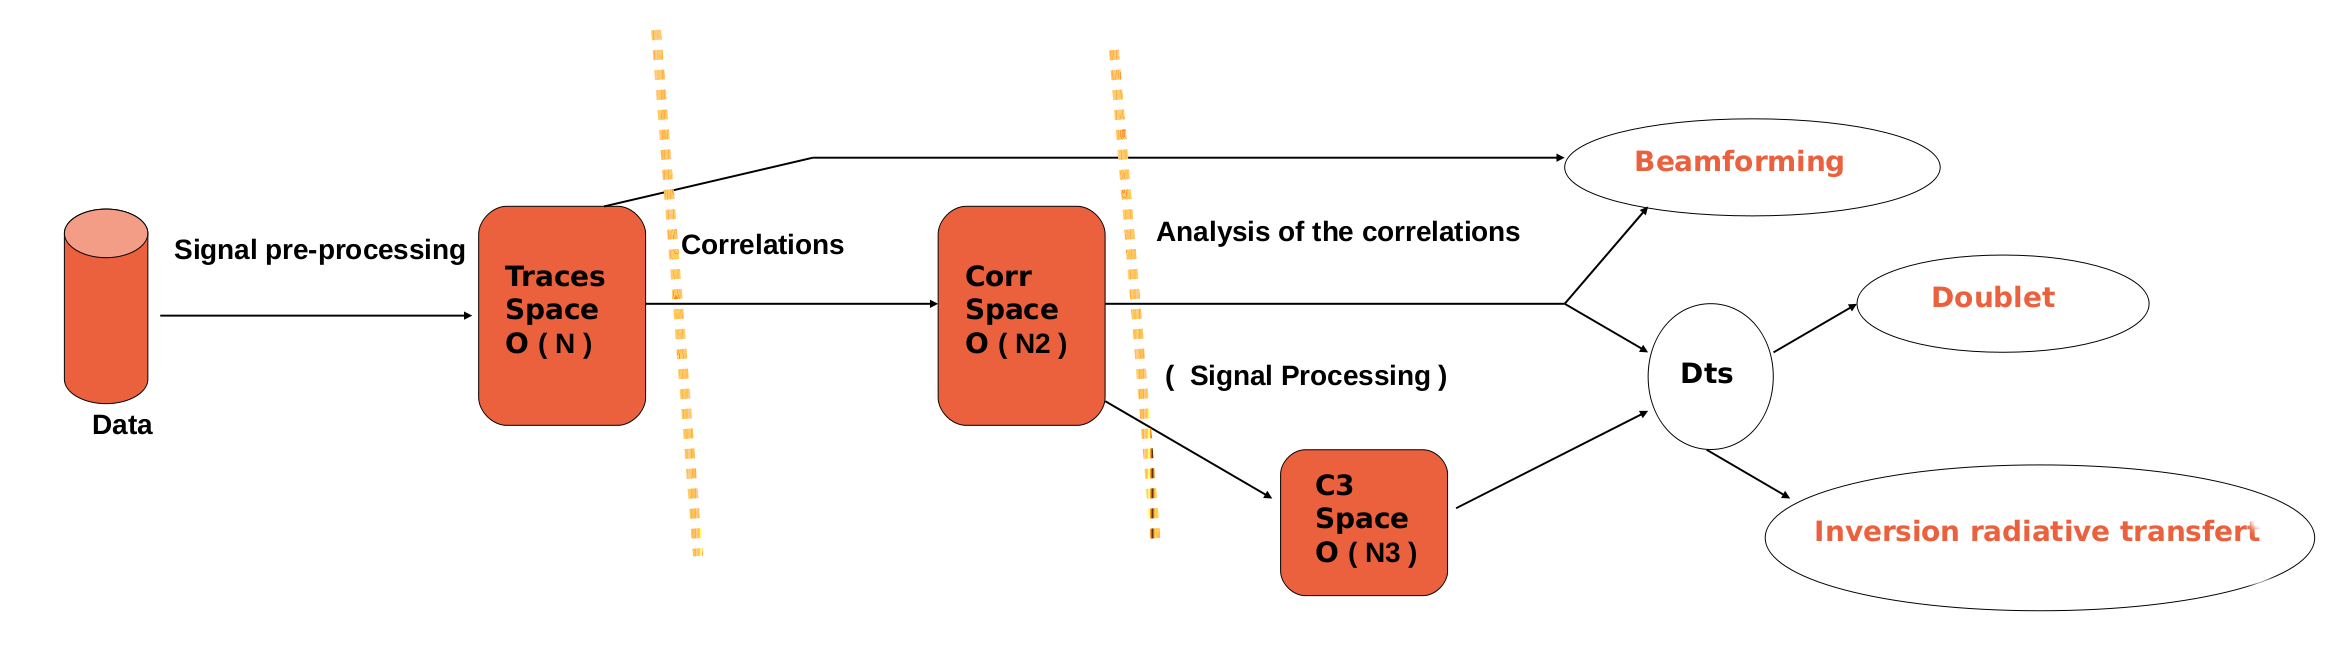
\includegraphics[width=16cm]{briandPosterAGU2013GimpProcessing.png}
\end{figure}


\newpage
\begin{multicols}{2}



\section{IT infrastrcuture for grid computing (6-12\S , 1-2 pages) }
~\\


The data-intensive processing
needs obviously an IT infrastructure in order to couple storage and computation.
In our cases, most of the processing are embarrassingly parallel.
The amount of data and the location of compute nodes available suggests using a 
distributed storage system with a grid manager.


The IT infrastructures used here are provided by the \emph{Ciment} \footnote{see ciment.ujf-grenoble.fr} 
platform. Ciment is the Grenoble University High Performance Computing (HPC) center. It offers a partial pooling of computing 
(6600 cores, plus GPU, 10 clusters) and many documentations for users. 
%It also provides a data grid environement : a grid of supercomputers and a distributed storage.
Moreover, the computational resources are integrated in a local grid, a grid of supercomputers. Associated with a distributed storage,
it provides a local data grid environement.

The distributed storage accessible by all the clusters is established and it is managed by iRODS \footnote{see irods.org}.
Nowadays it represents approximately 700 TB. Moreover, a grid management, the \emph{CiGri 
\footnote{see ciment.ujf-grenoble.fr/cigri/dokuwiki} middleware}, allows both access to iRODS storage and access 
to computing nodes of the clusters of the university (with the resource manager OAR \footnote{see oar.imag.fr}).


With Irods and CiGri, we can then access to the computational power of clusters of the University of Grenoble 
in mode best effort (with grid or parametric jobs). It may be noted that iRODS also acts to the user as a centralized controller with a 
total observation and thus allows the user to control its calculation.
~\\


The Integrated Rule-Oriented Data System (iRODS) is a data management software.
It permits to manage data independently the ressource storage with the i-commands or the iRODS API. 
It allows also the user to define metadata associated to the data (Collections) and make query on them
(see \cite{key:CCQSC} for an illustration of use). 
Moreover, it is a glass box, it is possible to define rules that call services (called microservices). One can define then automatic 
replication between differents ressources or more generally a processing for a selected data. 



The iRODS storage infrastructure of Ciment consists of a zone with the iCat server and several nodes, of the order of several tens,
see figure \ref{schemaCimentStorageNodesIcat}.

\begin{center}%[h]
\centering
\captionof{figure}{\label{schemaCimentStorageNodesIcat} iCAT and nodes storage}
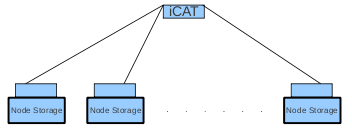
\includegraphics[width=6cm]{schemaCimentStorageNodesIcat.png}
\end{center}

Capacity has now reached 700 TB and is constantly evolving and increases with investment in new projects.
Each node comprises an Irods server coupled with further ressources as illustrated at the figure \ref{schemaNodeStorageCiment}

\begin{center}%[h]
\centering
\captionof{figure}{\label{schemaNodeStorageCiment} A node storage}
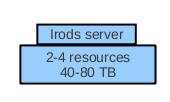
\includegraphics[width=3cm]{schemaNodeStorageCiment.png}
\end{center}

There is also a web interface where the user can check the status of the ressources (figure \ref{schemaCimentStorageStatus}).
The resources are grouped into three sites as near as possible of the supercomputers.
Note that one of the sites is 4km from the other two.

\begin{center}%[h]
\centering
\captionof{figure}{\label{schemaCimentStorageStatus}}
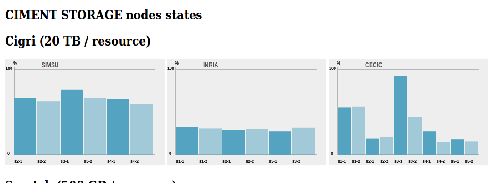
\includegraphics[width=8cm]{schemaCimentStorageStatus.png}
\end{center}

The access to 6600 cores of the clusters of the Ciment platform is achieved through the middleware CiGri.
Cigri launch jobs on idle processors of every computing clusters and then can optimize the resources usage.

Each cluster of the University of Grenoble uses the resource manager OAR. Cigri acts, among other things, as a metascheduler of OAR.
It retrieves the clusters states trough OAR and submits the jobs on free resources.

While it may work in normal mode, CiGri is used in BestEffort mode, ie that its jobs are lower priority: they can 
be killed by any other job. However, CiGri provides automatic resubmission. With this mecanism, the user can submit 
a big amount of small jobs, called a campaign, and he didn't care anymore.


Roughly speaking, in order to run a campaign, the user describes through a file (in json format) the parameters of the campaign 
such as the accepted cluters, the maximum duration, the location of the codes, and a prologue on each cluster in order to 
retrieve data and codes on iRODS. Moreover, it define also a file where each line correponds to a value of the parameter for the user's code.
Thus, the number of line of these parameter file corresponds to the number of jobs of the campaign.

Note that iRODS is accessible by all the nodes of all the clusters. By this way, for a given campaign, CiGri gets not only
the data to be process but also the codes to be run on the node. CiGri is therefore very independent of the data management of iRODS.

CiGri is now at the version 3, which represents a major evolution in terms of modeling and technology (Rest API, Ruby)

\newpage
\section{Results (28-31\S, 6-7 pages)}


\begin{thebibliography}{9}
\bibitem{key:CCQSC}
 Gen-Tao Chiang, Peter Clapham, Guoying Qi, Kevin Sale and Guy Coates,
 Implementing a genomic data management system using iRODS in the Wellcome Trust Sanger Institute.
{\em BMC Bioinformatics,12(1):361+, September 2011.}
\end{thebibliography}

\end{multicols}
\end{document}
